\documentclass[a4paper,12pt]{article}
%% Well understand input, and nice output
\usepackage[utf8]{inputenc}
\usepackage{lmodern}
\usepackage[T1]{fontenc}
\usepackage[english]{babel}

\usepackage{hyperref}
\hypersetup{colorlinks}  % uncomment this line if you prefer colored hyperlinks (e.g., for onscreen viewing)

% For graphics / images
\usepackage{graphicx}
\graphicspath{{graphics/}}
\DeclareGraphicsExtensions{.pdf,.eps,.png,.jpg}

\usepackage[left=0.5cm,right=0.5cm,top=1cm,bottom=1cm]{geometry}

\title{Test of LaTeX template to print Magic cards}

\begin{document}
\thispagestyle{empty}

% Magic Cards are this dimension
% 63mm x 88mm

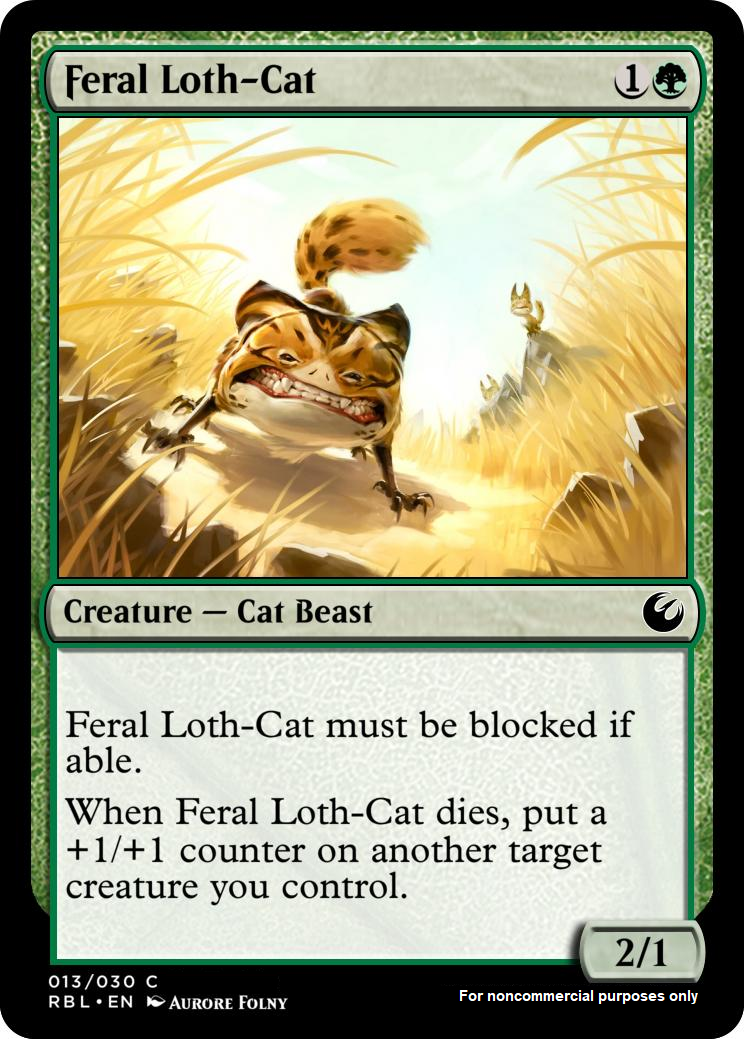
\includegraphics[width=63mm,height=88mm]{images/Feral_Loth-Cat.png}
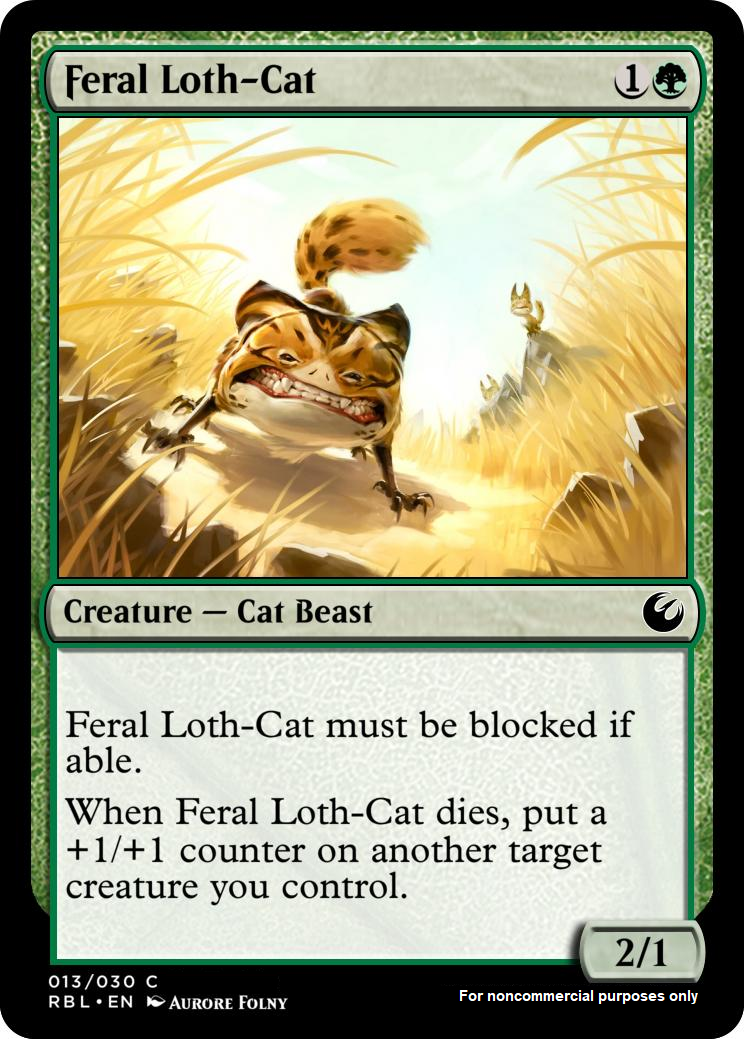
\includegraphics[width=63mm,height=88mm]{images/Feral_Loth-Cat.png}
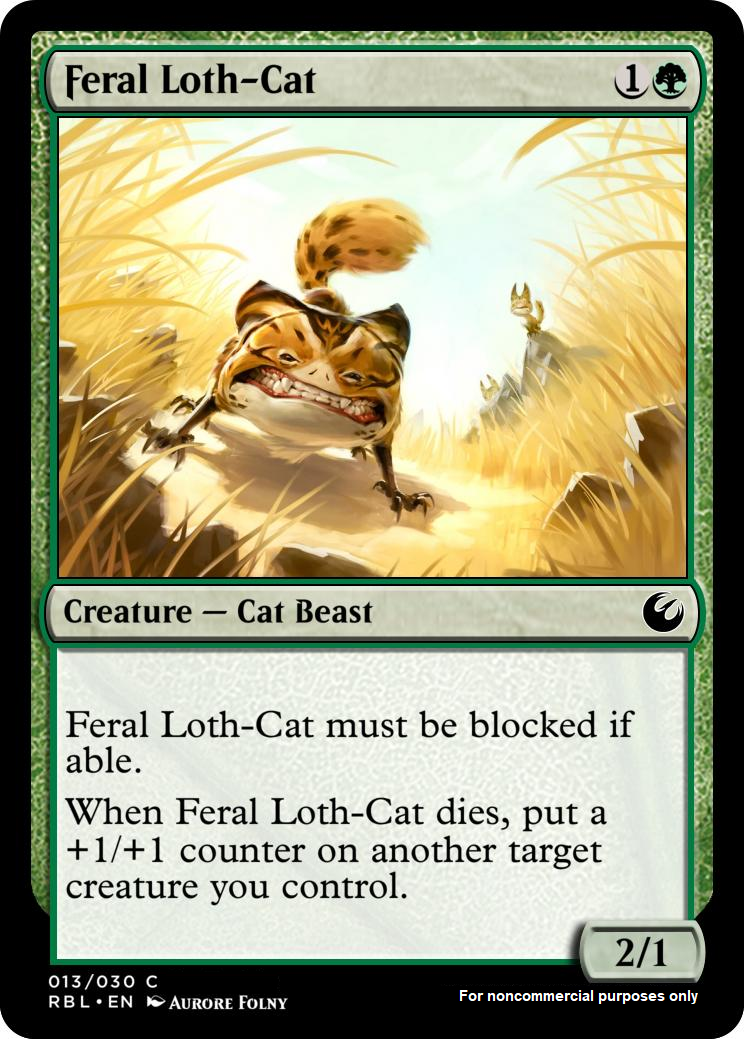
\includegraphics[width=63mm,height=88mm]{images/Feral_Loth-Cat.png}

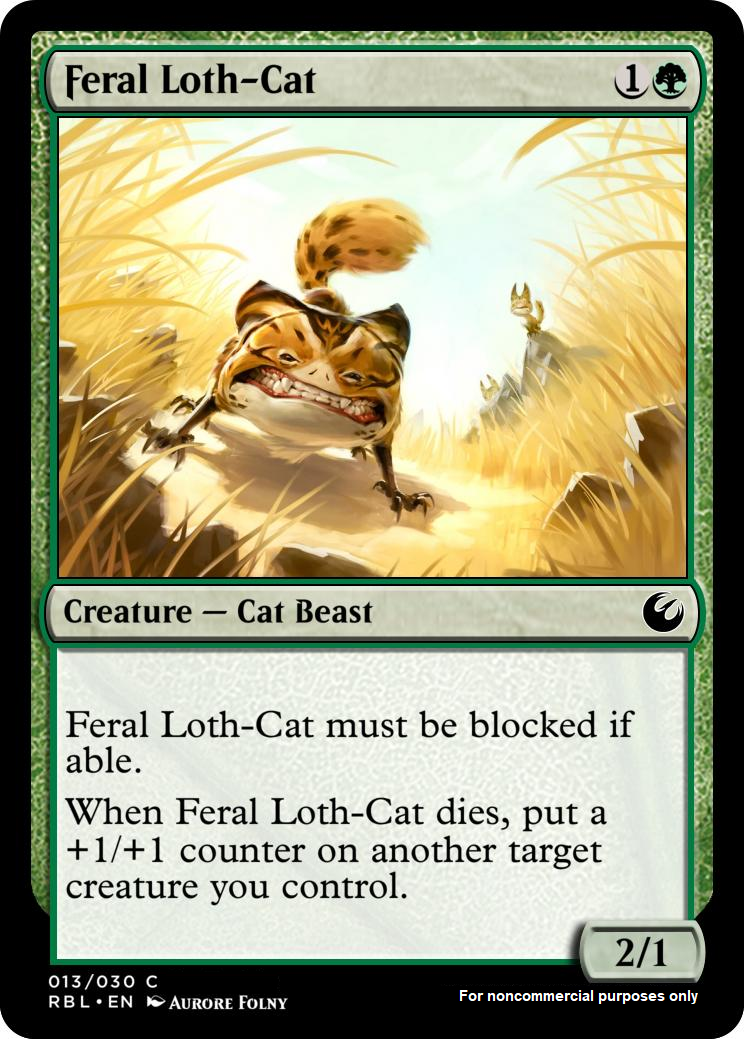
\includegraphics[width=63mm,height=88mm]{images/Feral_Loth-Cat.png}
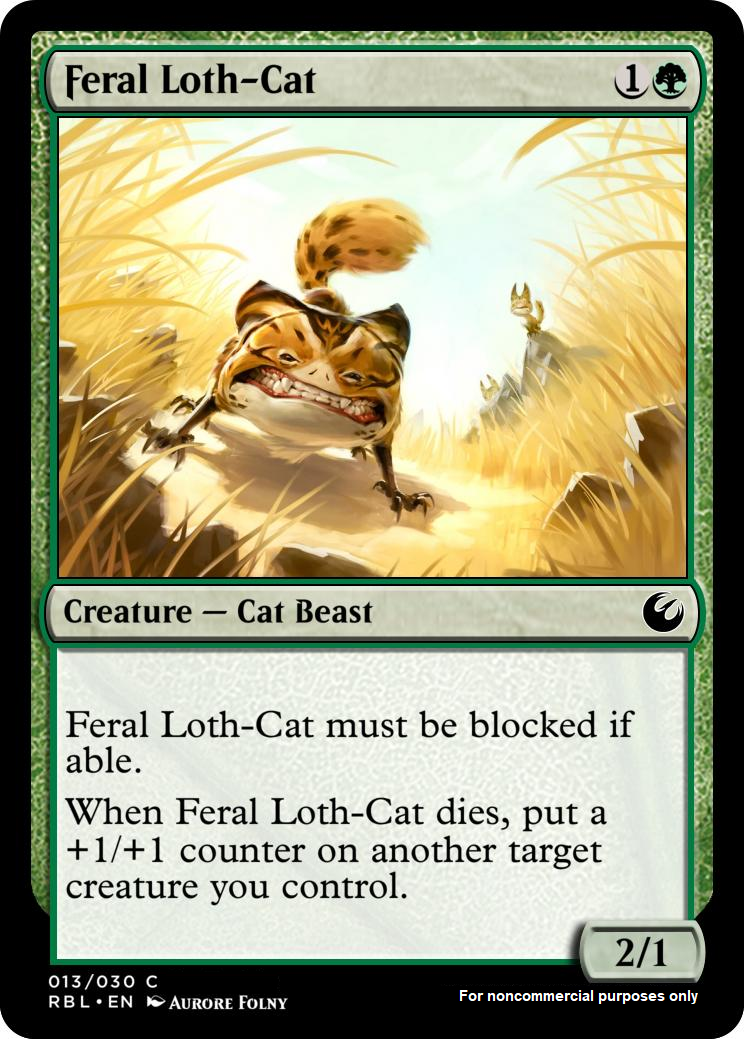
\includegraphics[width=63mm,height=88mm]{images/Feral_Loth-Cat.png}
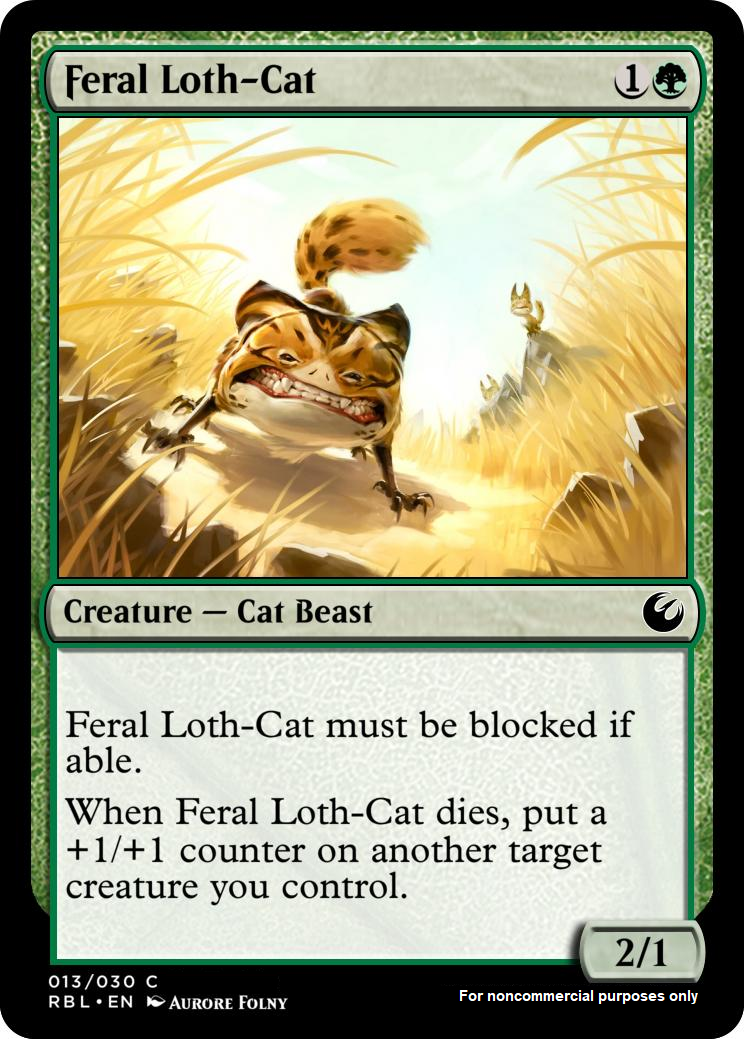
\includegraphics[width=63mm,height=88mm]{images/Feral_Loth-Cat.png}

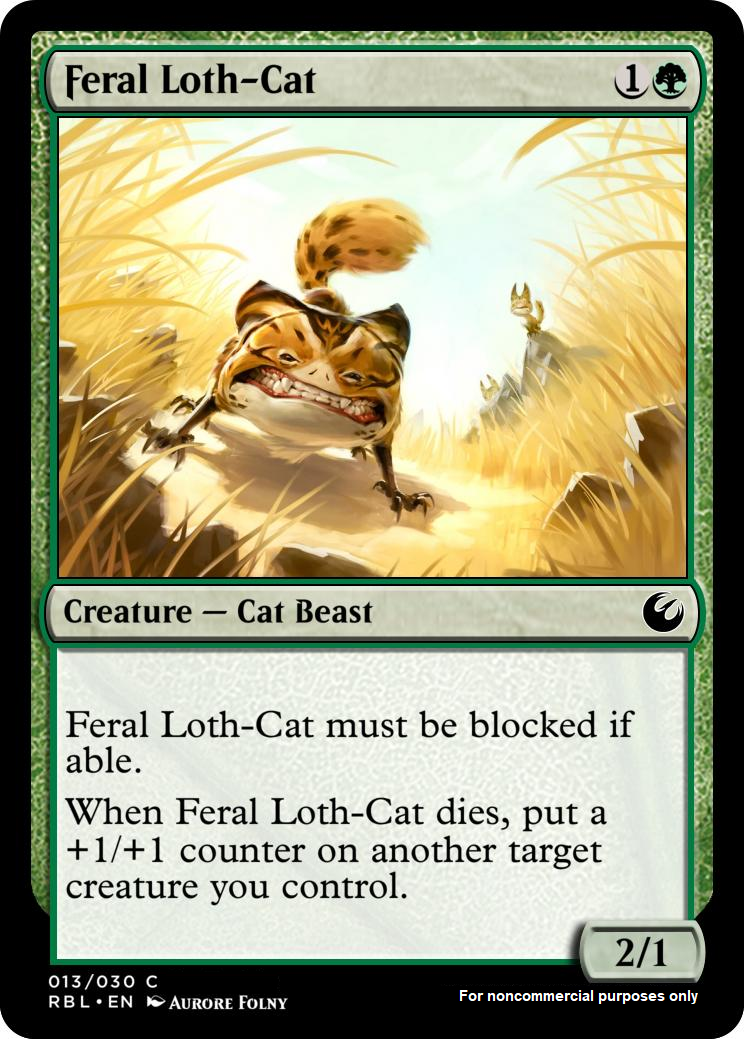
\includegraphics[width=63mm,height=88mm]{images/Feral_Loth-Cat.png}
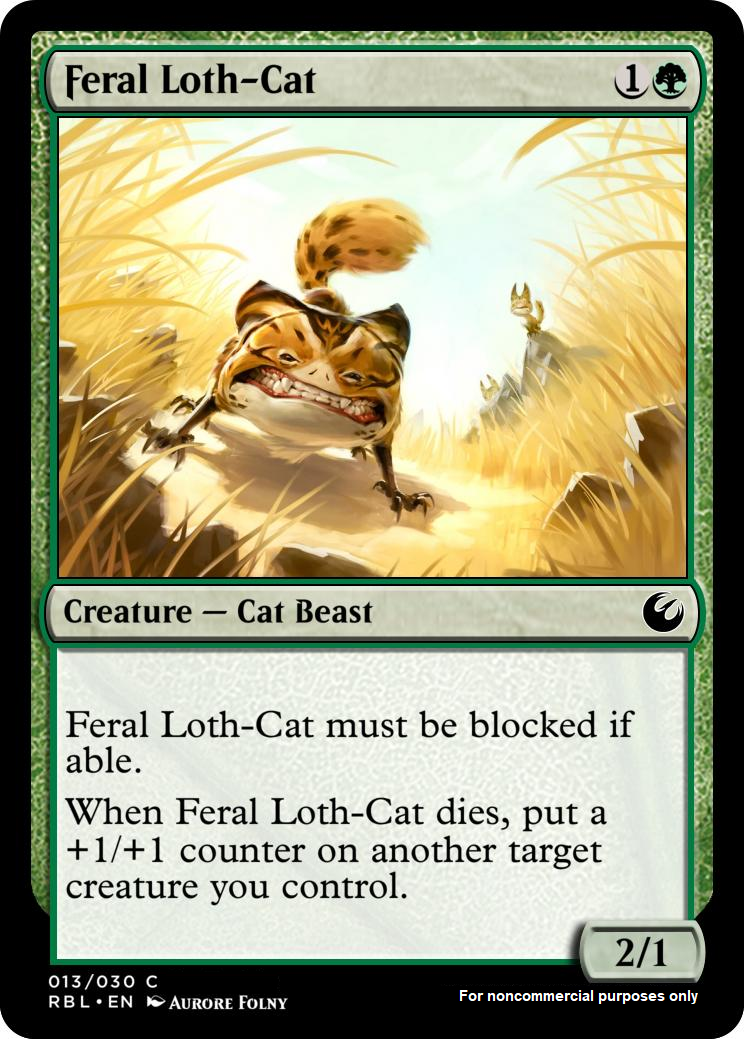
\includegraphics[width=63mm,height=88mm]{images/Feral_Loth-Cat.png}
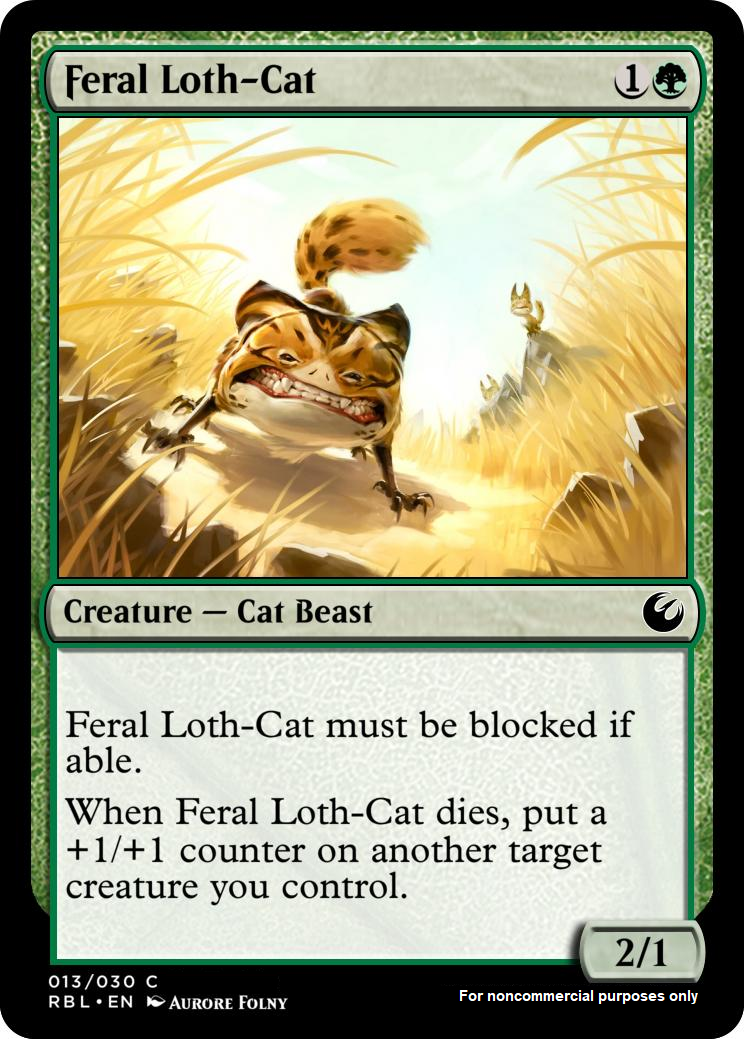
\includegraphics[width=63mm,height=88mm]{images/Feral_Loth-Cat.png}

\newpage

\end{document}
